\subsubsection{Modelado Guillermo Olvera} % (fold)
\label{ssub:ModeladoGuillermoOlvera}
    El modelo utiliza aut\'omatas celulares con la vecindad de Moore para simular la propagaci\'on y b\'usqueda de rutas del organismo 
        \textit{Physarum Polycephalum}. Este modelo funciona en una cuadr\'icula bidimensional donde cada c\'elula puede asumir 
        uno de varios estados: campo libre, nutriente no encontrado, repelente, punto inicial, gel en contracci\'on, 
        gel en compuesto, nutriente hallado, expansi\'on del \textit{Physarum} y gel sin compuesto.
    \vskip 0.5cm
    El algoritmo est\'a implementado en Python, lo cual introduce ciertas limitaciones en t\'erminos de 
        velocidad y escalabilidad. Debido a la naturaleza interpretada de Python, el modelo es lento 
        y poco escalable cuando se incrementa el n\'umero total de c\'elulas e hilos utilizados.
    \vskip 0.5cm
    El proceso comienza con la designaci\'on de una c\'elula inicial que representa el punto de inicio del \textit{Physarum}. 
        Las reglas de transici\'on determinan c\'omo cambian los estados de las c\'elulas en funci\'on de sus vecinos. Por ejemplo, 
        una c\'elula de campo libre se convierte en una c\'elula de expansi\'on del \textit{Physarum} si est\'a adyacente a una 
        c\'elula en estado de punto inicial, gel en contracci\'on o nutriente hallado. Las c\'elulas de expansi\'on del \textit{Physarum} 
        se propagan por la cuadr\'icula, y al encontrarse con nutrientes, estas c\'elulas cambian su estado a nutriente hallado, 
        lo que refuerza la ruta.
    \vskip 0.5cm
    \begin{figure}[h]
        \centering
        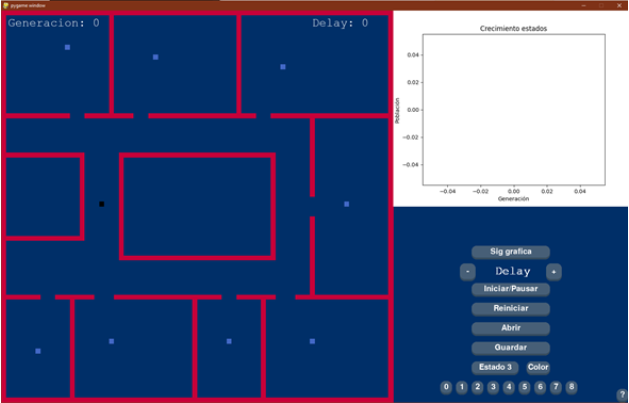
\includegraphics[width=0.5\textwidth]{./images/estado_del_arte/physarum/estadoInicialOlvera.png}
        \caption{Configuraci\'on inicial del \textit{Physarum} en la cuadr\'icula.}
        \label{fig:initial_state}
    \end{figure}
    \vskip 0.5cm
    A medida que el \textit{Physarum} se expande, se generan rutas que conectan las fuentes de nutrientes, 
        adapt\'andose din\'amicamente a la presencia de obst\'aculos y asegurando la conectividad en el entorno. Aunque el 
        algoritmo garantiza la formaci\'on de al menos una ruta viable, la trayectoria del \textit{Physarum} no es 
        realmente aleatoria, ya que sigue patrones determinados por las reglas de transici\'on. Estas reglas, sin embargo,
        no siempre son claras ni consistentes.
    \vskip 0.5cm
    \begin{figure}[h]
        \centering
        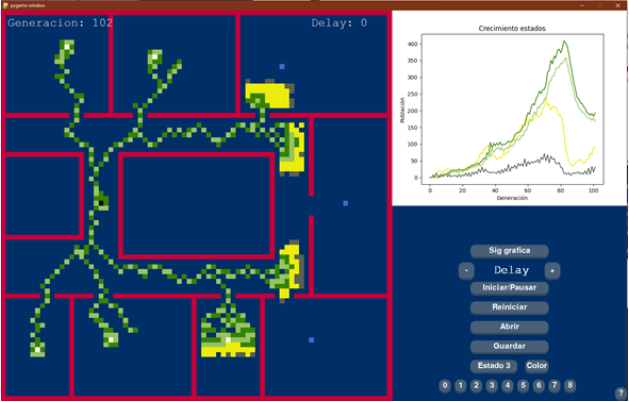
\includegraphics[width=0.5\textwidth]{./images/estado_del_arte/physarum/expansionOlvera.png}
        \caption{Expansi\'on del \textit{Physarum} y formaci\'on de rutas. \cite{Olvera2023}}
        \label{fig:expansion}
    \end{figure}
    \vskip 0.5cm
    Las reglas de transici\'on se definen para cada estado de la c\'elula, 
        asegurando que el \textit{Physarum} pueda encontrar y seguir rutas hacia los nutrientes, 
        adapt\'andose en tiempo real a cambios en el entorno. Sin embargo, estas reglas no 
        siempre son claras ni est\'an bien documentadas en la referencia \cite{Olvera2023}.

    % subsubsection Modelado Guillermo Olvera (end)